\documentclass{beamer}
 % \usetheme{metropolis}
% \usetheme{confposter}
\usepackage[orientation=portrait, size=a0, scale=1.4]{beamerposter}
\usepackage[utf8]{inputenc}
\usepackage[english]{babel}
\usepackage[T1]{fontenc}                                                                          
\usepackage{amsmath}
\usepackage{amsfonts}                                                                               
\usepackage{amssymb}
\usepackage{bm}
\usepackage{bbm}
\usepackage{subfig}
\usepackage{pgfplots}       
\usepackage[absolute,overlay]{textpos}

\definecolor{blkcol}{HTML}{E1E1EA}
\definecolor{blkcol2}{RGB}{209, 224, 224}
\definecolor{palered}{HTML}{FFD8D8}
\definecolor{darkprimcol}{HTML}{455A64}
\definecolor{lightprimcol}{HTML}{CFD8DC}
\definecolor{primcol}{HTML}{607D8B}
\definecolor{accentcol}{HTML}{448AFF}
\definecolor{primarytxt}{HTML}{212121}
\definecolor{secondtxt}{HTML}{757575}
\definecolor{dividertxt}{HTML}{BDBDBD}

\setbeamercolor{block title}{bg = blkcol}
\setbeamercolor{block body}{bg = blkcol!30}
\setbeamercolor{block body alerted}{bg = palered!50}
% \setbeamercolor{block title}{bg = darkprimcol, fg = white}
% \setbeamercolor{block body}{bg = lightprimcol}
% \setbeamercolor{block body alerted}{bg = accentcol!50}
\graphicspath{{../Slides/Figures/}}
%----------------------------------
\newlength{\sepwid}
\newlength{\onecolwid}
\newlength{\twocolwid}
\newlength{\threecolwid}
\newlength{\thirdcolwid}
\newlength{\leftmar}
\newlength{\centercol}
\setlength{\paperwidth}{36in} % A0 width: 46.8in
\setlength{\paperheight}{48in} % A0 height: 33.1in
\setlength{\leftmar}{0.035 \paperwidth}
\setlength{\sepwid}{0.005 \paperwidth} % Separation width (white space) between columns
\setlength{\sepwid}{0.01 \paperwidth} % Separation width (white space) between columns

\setlength{\onecolwid}{0.22\paperwidth} % Width of one column
\setlength{\twocolwid}{0.464\paperwidth} % Width of two columns
\setlength{\threecolwid}{0.708\paperwidth} % Width of three columns
\setlength{\topmargin}{-.2in} % Reduce the top margin size
\setlength{\thirdcolwid}{.301\paperwidth}
\setlength{\centercol}{0.93\paperwidth}
%------------------------------------
\newcommand{\Ex}{\mathbb{E}}
\newcommand{\Var}{\mathbb{V}\mathrm{ar}}
\newcommand{\Prob}{\mathbb{P}}
\DeclareMathOperator*{\argmin}{arg\,min}
\DeclareMathOperator*{\argmax}{arg\,max}
\newcommand{\Cov}{\textsf{Cov}}

\newcommand{\tra}{\mathrm{tr}}
\newcommand{\yobs}{\bm{y}^{\mathrm{obs}}}
\newcommand{\kest}{\hat{\bm{k}}}
\DeclareMathOperator*{\KL}{\textsf{KL}}


\setbeamertemplate{headline}{
 \leavevmode
  \begin{columns}
   \begin{column}{.02\linewidth}
   \end{column}
   \begin{column}{.58\linewidth}
    \vskip1cm
    \usebeamercolor{title in headline}{\color{fg}{\Huge\inserttitle}\\[1.5ex]}
    \usebeamercolor{author in headline}{\color{fg}{\insertauthor}\\[1ex]}
    \usebeamercolor{institute in headline}{\color{fg}\large{\insertinstitute}\\[0.1ex]}
    \vskip1cm
   \end{column}
   \begin{column}{.4\linewidth}
     
\includegraphics{INRIA_SCIENTIFIQUE_UK_CMJN}
     
\includegraphics{ljk}
   \end{column}
   \vspace{1cm}
  \end{columns}
 \vspace{0.5in}
 \hspace{0.5in}\begin{beamercolorbox}[wd=47in,colsep=0.15cm]{cboxb}\end{beamercolorbox}
 \vspace{0.1in}
}

\title{{\Huge \textbf{Parameter control in the presence of uncertainties}}}
\author{{\large \textbf{Victor Trappler},  Élise Arnaud, Laurent Debreu, Arthur Vidard} \\
  {\large \texttt{victor.trappler@univ-grenoble-alpes.fr}}}
\institute{\large AIRSEA Research team (Inria)-- Laboratoire Jean Kuntzmann \\
\textsc{Adjoint Workshop, Aveiro 2018}}
\titlegraphic{
\includegraphics[scale=1]{INRIA_SCIENTIFIQUE_UK_CMJN}

\includegraphics[scale=1]{ljk}}


\date{}

\begin{document}
\begin{frame}[t]
% \maketitle
\noindent\rule{\paperwidth}{1.5pt}
  \begin{columns}[t]
    \begin{column}{\leftmar}\end{column}
    \begin{column}{\centercol}

      
            \textbf{\Large How can one calibrate a computer model so that it performs reasonably well for different random operating conditions ?}

            
    \begin{alertblock}{Objectives}
      % Complex subgrid phenomena have to be parametrized in numerical models, and those values have to be properly estimated. This task is further complicated by the presence of uncertainties modelled by random variable. The calibrated value of the parameter is directly dependent on uncertainties.

      % Strategies taking into account those uncertainties are to be defined and applied on an academic model of a coastal area, in order to find an optimal value in a robust sense. 
    \begin{itemize}
    \item Define suitable \alert{definitions of robustness} in the field of computer code calibration
    \item Develop \alert{efficient} techniques and algorithms in order to estimate those parameters
    \item Deal with the high-dimension of the parameter spaces: \alert{Dimension reduction }
    \end{itemize}
  \end{alertblock}
\end{column}
\end{columns}

\begin{columns}[t] % The whole poster consists of three major columns, the second of which is split into two columns twice - the [t] option aligns each column's content to the top

\begin{column}{\leftmar}\end{column} % Empty spacer column

\begin{column}{\thirdcolwid} % The first column

  \begin{block}{Setting of the problem}
    % {\large Computer model: 2 inputs}
    %  \begin{itemize}
    % \item $\bm{k}\in\mathcal{K}$: the control/decision parameter
    % \item $\bm{u}\in\mathcal{U}$: the uncertain variable representing the environmental conditions
    % \end{itemize}  
    \begin{figure}[!h]
      \centering
      \resizebox{\linewidth}{!}{\begin{tikzpicture}
\usetikzlibrary{decorations.pathmorphing}

\definecolor{copper}{rgb}{0.69, 0.25, 0.21}
\definecolor{tin}{rgb}{0.7, 0.7, 0.7}

\tikzset{
  rugous1/.style = {black, thick,
    decoration={random steps,segment length=0.05cm,amplitude=.1cm}
  },
}
\tikzset{
  rugous2/.style = {black, thick,
    decoration={random steps,segment length=0.2cm,amplitude=.05cm}
  },
}
\tikzset{
  rugous3/.style = {black, thick,
    decoration={random steps,segment length=0.2cm,amplitude=.15cm}
  },
}

\filldraw [fill = blue!30]
   plot [samples = 100,domain = -5:5] (\x, {0.5*sin(\x r) + 2} )
-- plot [samples = 100,domain = 5:-5] (\x, {0.3*sin(\x/1.5 r)+0.5})
-- cycle;

\filldraw[fill = gray!30, draw = white]
   plot [samples = 100,domain = -5:5] (\x, {0.3*sin(\x/1.5 r)+0.5})
-- plot [samples = 100,domain = 5:-5] (\x, 0)
-- cycle;

\draw[rugous1, decorate](-5,0.52) -- (-2.3,0.2);
\draw[rugous2, decorate](-2.3,0.2) -- (2.4,0.8);
\draw[rugous3, decorate](2.4,0.8) -- (5,0.5);

\draw[->] (-5,0) -- (5,0);
\draw (0,0) node[below] {$x$};



\draw[->] (-5,0) -- (-5,3);

\draw[->] (0,0.5) -- (0,2);
\draw (0, 1.25) node[left] {$h(x,t)$} ;
\draw (0,0) node[below] {$x$};
\draw[->] (2,0) -- (2,{0.3*sin(2/1.5 r)+0.5});
\draw (2, 0.3) node[right] {$Z(x)$} ;
\draw[->] (1,0) -- (1,{0.5*sin(1 r)+2});
\draw (1, 1.3) node[right] {$H(x,t)$} ;
\end{tikzpicture}}
    \end{figure}
The calibration problem is to be able to find a value of $\bm{k}$ denoted $\kest$ that matches the best the observations $\yobs$. 
    
  \end{block}
\begin{block}{Inverse Problem}
  % \resizebox{\linewidth}{!}{\begin{tikzpicture}
\usetikzlibrary{decorations.pathmorphing}

\definecolor{copper}{rgb}{0.69, 0.25, 0.21}
\definecolor{tin}{rgb}{0.7, 0.7, 0.7}

\tikzset{
  rugous1/.style = {black, thick,
    decoration={random steps,segment length=0.05cm,amplitude=.1cm}
  },
}
\tikzset{
  rugous2/.style = {black, thick,
    decoration={random steps,segment length=0.2cm,amplitude=.05cm}
  },
}
\tikzset{
  rugous3/.style = {black, thick,
    decoration={random steps,segment length=0.2cm,amplitude=.15cm}
  },
}

\filldraw [fill = blue!30]
   plot [samples = 100,domain = -5:5] (\x, {0.5*sin(\x r) + 2} )
-- plot [samples = 100,domain = 5:-5] (\x, {0.3*sin(\x/1.5 r)+0.5})
-- cycle;

\filldraw[fill = gray!30, draw = white]
   plot [samples = 100,domain = -5:5] (\x, {0.3*sin(\x/1.5 r)+0.5})
-- plot [samples = 100,domain = 5:-5] (\x, 0)
-- cycle;

\draw[rugous1, decorate](-5,0.52) -- (-2.3,0.2);
\draw[rugous2, decorate](-2.3,0.2) -- (2.4,0.8);
\draw[rugous3, decorate](2.4,0.8) -- (5,0.5);

\draw[->] (-5,0) -- (5,0);
\draw (0,0) node[below] {$x$};



\draw[->] (-5,0) -- (-5,3);

\draw[->] (0,0.5) -- (0,2);
\draw (0, 1.25) node[left] {$h(x,t)$} ;
\draw (0,0) node[below] {$x$};
\draw[->] (2,0) -- (2,{0.3*sin(2/1.5 r)+0.5});
\draw (2, 0.3) node[right] {$Z(x)$} ;
\draw[->] (1,0) -- (1,{0.5*sin(1 r)+2});
\draw (1, 1.3) node[right] {$H(x,t)$} ;
\end{tikzpicture}}
\begin{figure}[!h]
  \centering
  {\usetikzlibrary{positioning}

\tikzstyle{block} = [rectangle, draw, fill=mist, 
    text centered, minimum width=10em, text = white] 
%  \tikzstyle{block} = [rectangle, draw, fill=blkcol, 
%       text centered, minimum width=3em]

% \tikzstyle{block2} = [rectangle, draw, fill=blkcol2, 
%      text centered, rounded corners, minimum width=3em]
% 
% \tikzstyle{block2} = [rectangle, draw, fill=blkcol2, 
%      text centered, rounded corners, minimum width=3em]

\tikzstyle{LHS}=[rectangle, draw, text centered]
\begin{tikzpicture}[node distance= 2em]

%\node [align = center] at (0,0) (input) {Control variable \\$\mathbf{k} \in \mathcal{K}$};
\node [align = center] (input) {Control variable \\$\bm{k} \in \mathcal{K}$};
\node[block ,right =  of input] (code){Direct Simulation};
%\node [align = center, above =of  code ] (envir) {Environmental variables \\$\mathbf{u} \in \mathcal{U}$ fixed};
\node [align = center, above = of code] (envir) {Environmental variables \\ \emph{$\bm{U} \in \mathcal{U}$ random}};




%\node[align = center, right =of  code] (output) {$W(\mathbf{k})$};
\node[align = center, right = of code]  (output) {\emph{$M(\bm{k},\bm{u})$}};
%\node [align = center, right =of  inv, below = of output]  (obs) {$\mathbf{y}$};
\node[block, below =of code] (inv) {Inverse Problem};
\node [align = center, right = of inv,  below =  of output] (obs) {$\bm{y}_{\mathrm{obs}}$};

\draw[->] (input) -- (code);
\draw[->] (envir) -- (code);
\draw[->] (code) -- (output);

 % \node [align = center] at (0,0) (input) {$Y = \mathcal{H}W(K_{\mathrm{ref}})$};
 % \node [align = center] at (4,1.5) (envir) {Environmental variables \\$X_e$ r.v.};

 % \node[block] at (4,0)(code){"Inverse Problem"};

% \node[align = center] at (8,0) (output) {$K$};

\draw[->] (input) -- (code);
% \draw[->] (envir) -- (code);
\draw[->] (code) -- (output);
\draw[->] (output) -- (obs) ;
\draw[->] (inv) -|(input) ;
\draw[->] (obs) -- (inv);
\end{tikzpicture}
}
\end{figure}
    
% \usetikzlibrary{positioning}
\tikzstyle{block} = [rectangle, draw, fill=blue!30, 
    text centered, minimum width=10em] 
%  \tikzstyle{block} = [rectangle, draw, fill=blkcol, 
%       text centered, minimum width=3em]

% \tikzstyle{block2} = [rectangle, draw, fill=blkcol2, 
%      text centered, rounded corners, minimum width=3em]
% 
% \tikzstyle{block2} = [rectangle, draw, fill=blkcol2, 
%      text centered, rounded corners, minimum width=3em]

\tikzstyle{LHS}=[rectangle, draw, text centered]
\begin{center}
\begin{tikzpicture}[node distance= 2em]

%\node [align = center] at (0,0) (input) {Control variable \\$\bm{k} \in \mathcal{K}$};
\node [align = center]  (input) {Control variable \\$\bm{k} \in \mathcal{K}$};
\node[block ,right =  of input](code){Direct Simulation};
%\node [align = center, above =of  code ] (envir) {Environmental variables \\$\mathbf{u} \in \mathcal{U}$ fixed};
\node [align = center, above = of code] (envir) {Environmental variables \\$\bm{u} \in \mathcal{U}$ fixed};





\node[align = center, right = of code]  (output) {$M(\bm{k})$}; 
\node[block, below =of code] (inv) {Inverse Problem};
\node [align = center, right = of inv,  below =  of output] (obs) {$\yobs$};

\draw[->] (input) -- (code);
\draw[->] (envir) -- (code);
\draw[->] (code) -- (output);

 % \node [align = center] at (0,0) (input) {$Y = \mathcal{H}W(K_{\mathrm{ref}})$};
 % \node [align = center] at (4,1.5) (envir) {Environmental variables \\$X_e$ r.v.};

 % \node[block] at (4,0)(code){"Inverse Problem"};

% \node[align = center] at (8,0) (output) {$K$};

\draw[->] (input) -- (code);
% \draw[->] (envir) -- (code);
\draw[->] (code) -- (output);
\draw[->] (output) -- (obs) ;
\draw[->] (inv) -|(input) ;
\draw[->] (obs) -- (inv);
\end{tikzpicture}
\end{center}
    \begin{equation*}
      \tag{Cost function}
  J(\bm{k}) = \frac12 \|M(\bm{k}) - \yobs \|_{\bm\Sigma^{-1}}^2 
\end{equation*}
and we have to perform the following minimisation problem, usually with the help of the adjoint method
\begin{equation*}
  \kest = \argmin_{\bm{k}\in\mathcal{K}} J(\bm{k})
\end{equation*}

Now, $\bm{u} \text{ sampled from } \bm{U} \text{ of density } p_U$
and $\yobs = M(\bm{k}_{\mathrm{ref}}, \bm{u}_{\mathrm{ref}})$
% \newline

% \resizebox{.8\linewidth}{!}{\usetikzlibrary{positioning}

\tikzstyle{block} = [rectangle, draw, fill=mist, 
    text centered, minimum width=10em, text = white] 
%  \tikzstyle{block} = [rectangle, draw, fill=blkcol, 
%       text centered, minimum width=3em]

% \tikzstyle{block2} = [rectangle, draw, fill=blkcol2, 
%      text centered, rounded corners, minimum width=3em]
% 
% \tikzstyle{block2} = [rectangle, draw, fill=blkcol2, 
%      text centered, rounded corners, minimum width=3em]

\tikzstyle{LHS}=[rectangle, draw, text centered]
\begin{tikzpicture}[node distance= 2em]

%\node [align = center] at (0,0) (input) {Control variable \\$\mathbf{k} \in \mathcal{K}$};
\node [align = center] (input) {Control variable \\$\bm{k} \in \mathcal{K}$};
\node[block ,right =  of input] (code){Direct Simulation};
%\node [align = center, above =of  code ] (envir) {Environmental variables \\$\mathbf{u} \in \mathcal{U}$ fixed};
\node [align = center, above = of code] (envir) {Environmental variables \\ \emph{$\bm{U} \in \mathcal{U}$ random}};




%\node[align = center, right =of  code] (output) {$W(\mathbf{k})$};
\node[align = center, right = of code]  (output) {\emph{$M(\bm{k},\bm{u})$}};
%\node [align = center, right =of  inv, below = of output]  (obs) {$\mathbf{y}$};
\node[block, below =of code] (inv) {Inverse Problem};
\node [align = center, right = of inv,  below =  of output] (obs) {$\bm{y}_{\mathrm{obs}}$};

\draw[->] (input) -- (code);
\draw[->] (envir) -- (code);
\draw[->] (code) -- (output);

 % \node [align = center] at (0,0) (input) {$Y = \mathcal{H}W(K_{\mathrm{ref}})$};
 % \node [align = center] at (4,1.5) (envir) {Environmental variables \\$X_e$ r.v.};

 % \node[block] at (4,0)(code){"Inverse Problem"};

% \node[align = center] at (8,0) (output) {$K$};

\draw[->] (input) -- (code);
% \draw[->] (envir) -- (code);
\draw[->] (code) -- (output);
\draw[->] (output) -- (obs) ;
\draw[->] (inv) -|(input) ;
\draw[->] (obs) -- (inv);
\end{tikzpicture}
}
% \framebox{\resizebox{0.5\linewidth}{!}{\usetikzlibrary{positioning}

\tikzstyle{block} = [rectangle, draw, fill=mist, 
    text centered, minimum width=10em, text = white] 
%  \tikzstyle{block} = [rectangle, draw, fill=blkcol, 
%       text centered, minimum width=3em]

% \tikzstyle{block2} = [rectangle, draw, fill=blkcol2, 
%      text centered, rounded corners, minimum width=3em]
% 
% \tikzstyle{block2} = [rectangle, draw, fill=blkcol2, 
%      text centered, rounded corners, minimum width=3em]

\tikzstyle{LHS}=[rectangle, draw, text centered]
\begin{tikzpicture}[node distance= 2em]

%\node [align = center] at (0,0) (input) {Control variable \\$\mathbf{k} \in \mathcal{K}$};
\node [align = center] (input) {Control variable \\$\bm{k} \in \mathcal{K}$};
\node[block ,right =  of input] (code){Direct Simulation};
%\node [align = center, above =of  code ] (envir) {Environmental variables \\$\mathbf{u} \in \mathcal{U}$ fixed};
\node [align = center, above = of code] (envir) {Environmental variables \\ \emph{$\bm{U} \in \mathcal{U}$ random}};




%\node[align = center, right =of  code] (output) {$W(\mathbf{k})$};
\node[align = center, right = of code]  (output) {\emph{$M(\bm{k},\bm{u})$}};
%\node [align = center, right =of  inv, below = of output]  (obs) {$\mathbf{y}$};
\node[block, below =of code] (inv) {Inverse Problem};
\node [align = center, right = of inv,  below =  of output] (obs) {$\bm{y}_{\mathrm{obs}}$};

\draw[->] (input) -- (code);
\draw[->] (envir) -- (code);
\draw[->] (code) -- (output);

 % \node [align = center] at (0,0) (input) {$Y = \mathcal{H}W(K_{\mathrm{ref}})$};
 % \node [align = center] at (4,1.5) (envir) {Environmental variables \\$X_e$ r.v.};

 % \node[block] at (4,0)(code){"Inverse Problem"};

% \node[align = center] at (8,0) (output) {$K$};

\draw[->] (input) -- (code);
% \draw[->] (envir) -- (code);
\draw[->] (code) -- (output);
\draw[->] (output) -- (obs) ;
\draw[->] (inv) -|(input) ;
\draw[->] (obs) -- (inv);
\end{tikzpicture}
}}


The loss function is now
\begin{equation*}
  \underbrace{J(\bm{k},\alert{\bm{U}}) = \frac12 \|M(\bm{k},\alert{\bm{U}}) - \yobs \|_{\bm\Sigma^{-1}}^2}_{\text{Random variable}}
\end{equation*}

\begin{itemize}
\item What criteria to use to ``optimize'' in a sense $J$ ?
\item How to deal with long computation ?
\end{itemize}
% \begin{itemize}
% \item Risk/Utility approach \cite{lehman_designing_2004}: minimize a statistical moment of $J(\bm{k},\bm{U})$:
%   \begin{equation*}
%     \min_{\bm{k}} \Ex_U[J(\bm{k},\bm{U})] \quad  \min_{\bm{k}} \Var_U[J(\bm{k},\bm{U})]
%   \end{equation*}
% \item Bayesian approach \cite{tarantola_inverse_2005}, $J$ is linked to the joint likelihood of $\bm{k}$ and $\bm{u}$ by:
%   \begin{equation*}
%     p_{Y|K,U}(y|\bm{k},\bm{u}) \propto \exp\left[-J(\bm{k},\bm{u}) \right]
%   \end{equation*}
% \end{itemize}
\end{block}
\begin{block}{Which criterion to choose ? \cite{lehman_designing_2004,janusevskis_simultaneous_2010}}
  Different approaches
  \begin{itemize}
  \item Consider the \alert{worst-case scenario} \cite{wald_statistical_1945}
    \begin{align*}
      J_{\mathrm{w}}(\bm{k}) = \max_{\bm{u}\in\mathcal{U}} J(\bm{k},\bm{u}) \quad \text{ and } \quad \kest_{\mathrm{wc}} = \argmin_{\bm{k}} J_{\mathrm{w}}(\bm{k})
    \end{align*}
    \item The solution gives \alert{good results on average}:
  \begin{align*}
    \mu(\bm{k}) = \Ex_U[J(\bm{k},\bm{U})]\quad \text{ and }  \quad  \kest_{\mu} = \argmin_{\bm{k}}  \mu(\bm{k})
  \end{align*}

 \item The estimate gives \alert{steady results}:
  \begin{align*}
    \sigma^2(\bm{k}) = \Var_U[J(\bm{k},\bm{U})] \quad\text{ and } \quad \kest_{\sigma^2} = \argmin_{\bm{k}} \sigma^2(\bm{k})
  \end{align*}

  % \begin{align*} 
  %   \kest_{\mu} &= \argmin_{\bm{k}}  \mu(\bm{k}) \\
  %   \kest_{\sigma^2} &= \argmin_{\bm{k}} \sigma^2(\bm{k})
                         %     \end{align*}
 
  \item \alert{Compromise} between Mean and Variance: multiobjective optimization problem:
  \begin{align*}
    \text{Pareto front of } (\mu(\bm{k}),\sigma^2(\bm{k}))
  \end{align*}
\item Reliability analysis: \alert{Probability of being below threshold} $T$
  \begin{align*}
    R_T(\bm{k}) =  \Prob\left[J(\bm{k},\bm{U}) \leq T\right], \quad \kest_{R_T} = \argmax R_T(\bm{k})
  \end{align*}
\item Special case: $T_{\min} = T(\bm{U}) = \min_{\bm{k}} J(\bm{k},\bm{U})$
  \begin{align*}
    \Prob\left[J(\bm{k},\bm{U}) \leq T_{\min}\right] = \Prob\left[\bm{k} = \argmin_{\tilde{\bm{k}}} J(\tilde{\bm{k}},\bm{U}) \right]
  \end{align*}
\end{itemize}
\end{block}
\end{column}

\begin{column}{\sepwid}\end{column} % Empty spacer column

\begin{column}{\thirdcolwid} % Begin a column which is two columns wide (column 2)


%
  \begin{block}{Bayesian approach}
    Include beliefs upon $\bm{K}$ and $\bm{U}$ through priors:
Bayes' theorem
  \begin{align*}
    p_{K,U|Y}(\bm{k},\bm{u}|\yobs) &\propto p_U(\bm{u}) p_K(\bm{k}) \overbrace{p_{Y|K,U}(y|\bm{k},\bm{u})}^{\exp(-J(\bm{k},\bm{u}))} \\
                                   &\propto p_U(\bm{u})  \underbrace{\alert{p_{K|Y,U}(\bm{k}|\yobs,\bm{u})}}_{ = f(\bm{k},\bm{u}) }
  \end{align*}

  
  
  % Let us then define a family of densities: \begin{align*}\{\bm{k} \mapsto p_{K|Y,U}(\bm{k}|\yobs,\bm{u}) = f(\bm{k},\bm{u}), \bm{u} \in \mathcal{U}\}\end{align*}
  % and that yield the following estimates
% \begin{itemize}
% \item $\begin{aligned}[t]\kest_{\mathrm{MMAP}}  &= \argmax p_{K|Y}(\bm{k}|\yobs)\end{aligned}$
% \item $\begin{aligned}[t]\kest_{\sigma} = \argmin_{\bm{k}} \Var_U[p_{K|Y,U}(\bm{k}|\yobs,\bm{u})]\end{aligned}$
% \item $\begin{aligned}[t]\kest_{\mathrm{wc}} = \argmax_{\bm{k}} \{ \min_{\bm{u}}p_{K|Y,U}(\bm{k}|\yobs,\bm{u}) \}\end{aligned} $
% \item Given a threshold $T$, study the probability of exceedance $p_{K_T}(\bm{k}) = \Prob\left[p_{K|Y,U}(\bm{k}|\yobs,\bm{U})\geq T \right]$
% \item Special case: $T = \max_{\bm{k}} p_{K|Y,U}(\bm{k}|\yobs,\bm{U})$.


%   Study $\bm{K}_{\argmax} = \argmax_{\bm{k}} p_{K|Y,U}(\bm{k}|\yobs,\bm{U})$, a random variable
% \item $p_{\argmax}(\bm{k}) = \Ex_U\left[ \mathbbm{1}_{\{p(\bm{k}|\yobs,\bm{U})>p(\tilde{\bm{k}}|\yobs,\bm{U}),\forall \tilde{\bm{k}}\}}\right]$
% \end{itemize}

% \begin{itemize}
% \item $\begin{aligned}[t]\kest_{\mathrm{MMAP}}  &= \argmax p_{K|Y}(\bm{k}|\yobs)\\ &= \argmax \int f(\bm{k},\bm{u}) p_U(\bm{u})\,\mathrm{d}\bm{u}\end{aligned}$
% \item $\begin{aligned}[t]\kest_{\sigma} = \argmin_{\bm{k}} \Var_U[f(\bm{k},\bm{u})]\end{aligned}$
% \item $\begin{aligned}[t]\kest_{\mathrm{wc}} = \argmax_{\bm{k}} \{ \min_{\bm{u}}f(\bm{k},\bm{u}) \}\end{aligned} $
% \item Given a threshold $T$, study the probability of exceedance $p_{K_T}(\bm{k}) = \Prob\left[f(\bm{k},\bm{U})\geq T \right]$
% \item Special case: $T_{\max}(\bm{U}) = \max_{\bm{k}} f(\bm{k},\bm{U})$.


%   Study $\bm{K}_{\argmax} = \argmax_{\bm{k}} p_{K|Y,U}(\bm{k}|\yobs,\bm{U})$, a random variable
% % \item $p_{\argmax}(\bm{k}) = \Ex_U\left[ \mathbbm{1}_{\{p(\bm{k}|\yobs,\bm{U})>p(\tilde{\bm{k}}|\yobs,\bm{U}),\forall \tilde{\bm{k}}\}}\right]$
% \end{itemize}

% \begin{figure}[!h]
%       \centering
%       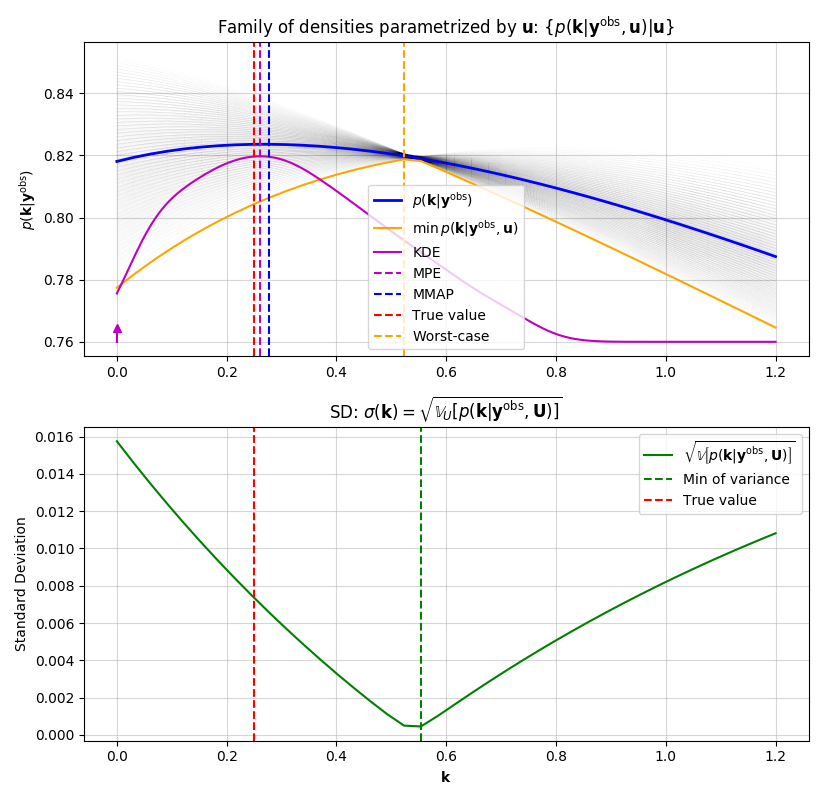
\includegraphics[width = .95\linewidth]{MMAP_minvariance}
%       \caption{Family of densities, and estimates obtained in $\dim \mathcal K$ = 1}
%     \end{figure}

    \begin{figure}[!h]
      \centering
      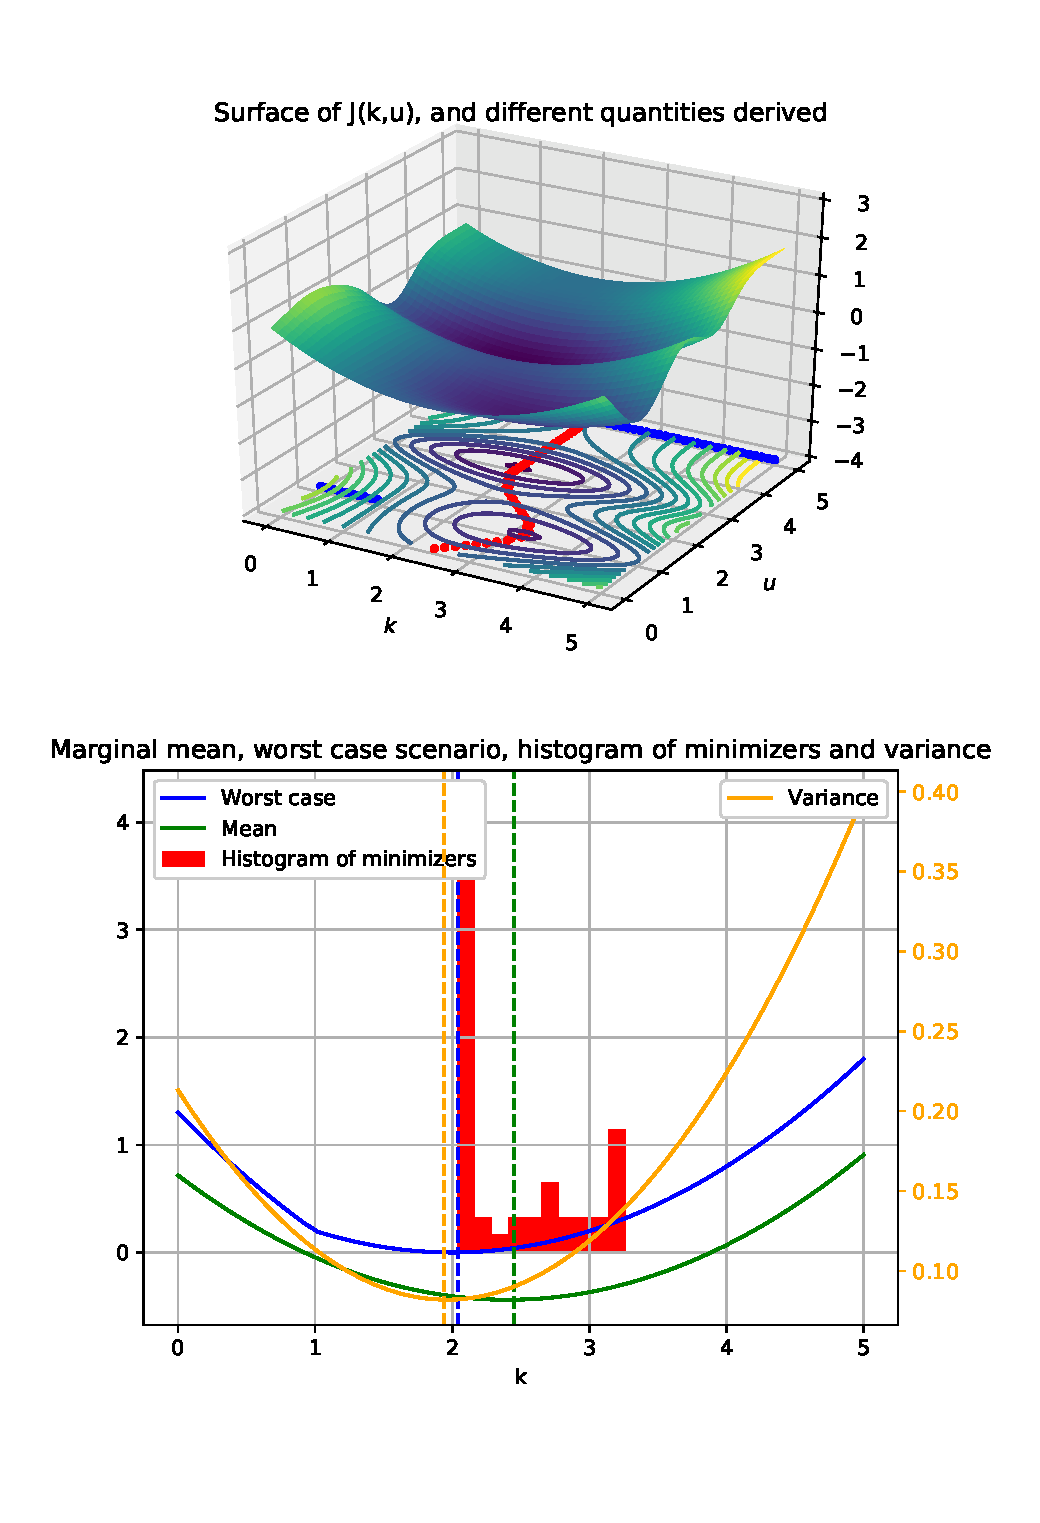
\includegraphics[width = \linewidth]{Surface}
    \end{figure}
  \end{block}

  

%----------------------------------------------------------------------------------------

\begin{block}{Methods}
  \begin{itemize}
  \item \alert{MCMC based methods} to sample from the posterior distribution $p_{K,U|Y}(\bm{k},\bm{u}|\yobs)$, and/or marginalize
    \begin{itemize}
    \item State Augmentation for Marginal Estimation (SAME) \cite{doucet_marginal_2002} to get $\kest_{\mathrm{MMAP}}$
    \item Hamiltonian/Langevin Monte Carlo: Improve convergence of MCMC via the information brought by the gradient of the posterior.
    \end{itemize}
  \item Estimation of \alert{$\bm{K}_{\argmax}$}
    \begin{itemize}
    \item Need for efficient optimization (importance of the gradient)
    \item Kernel Density Estimation
    \item Clustering/ Mode-seeking algorithms
    \end{itemize}


  \item Metamodelling
\begin{itemize}
  \item Build surrogate model cheap to evaluate
  \item Lead to adaptative sampling strategies
  \end{itemize}
  \end{itemize}
\end{block}
% ----------------------------------------------------------------------------------

%----------------------------------------------------------------------------------------

\end{column} % End of column 2

\begin{column}{\sepwid}\end{column} % Empty spacer column

%----------------------------------------------------------------------------------------
%	MATHEMATICAL SECTION
%----------------------------------------------------------------------------------------
\begin{column}{\thirdcolwid} % Column 3


%------------------------------------------------------------------------------------
\begin{block}{Avoid MCMC by studying $\bm{K}_{\argmax}$}
  \begin{itemize}
  \item Sample $\bm{u}^{(i)}$ from $\bm{U}$ of density $p_U$.
  \item Using adjoint method, 
    \begin{equation*}
      \bm{k}_{\argmax}^{(i)} = \argmax p_{K|Y,U}(\bm{k}|\yobs, \bm{u}^{(i)})
    \end{equation*}
  \item Once the set of samples $(\bm{k}_{\argmax}^{(i)})$ is sufficient
    \begin{itemize}
    \item Either KDE and perform a direct optimization on the estimate
    \item Either perform Clustering analysis
    \end{itemize}
  \end{itemize}
\end{block}
%----------------------------------------------------------------------------------------
%----------------------------------------------------------------------------------------

%----------------------------------------------------------------------------------------
%	RESULTS
%----------------------------------------------------------------------------------------

\begin{block}{Results}

\begin{figure}
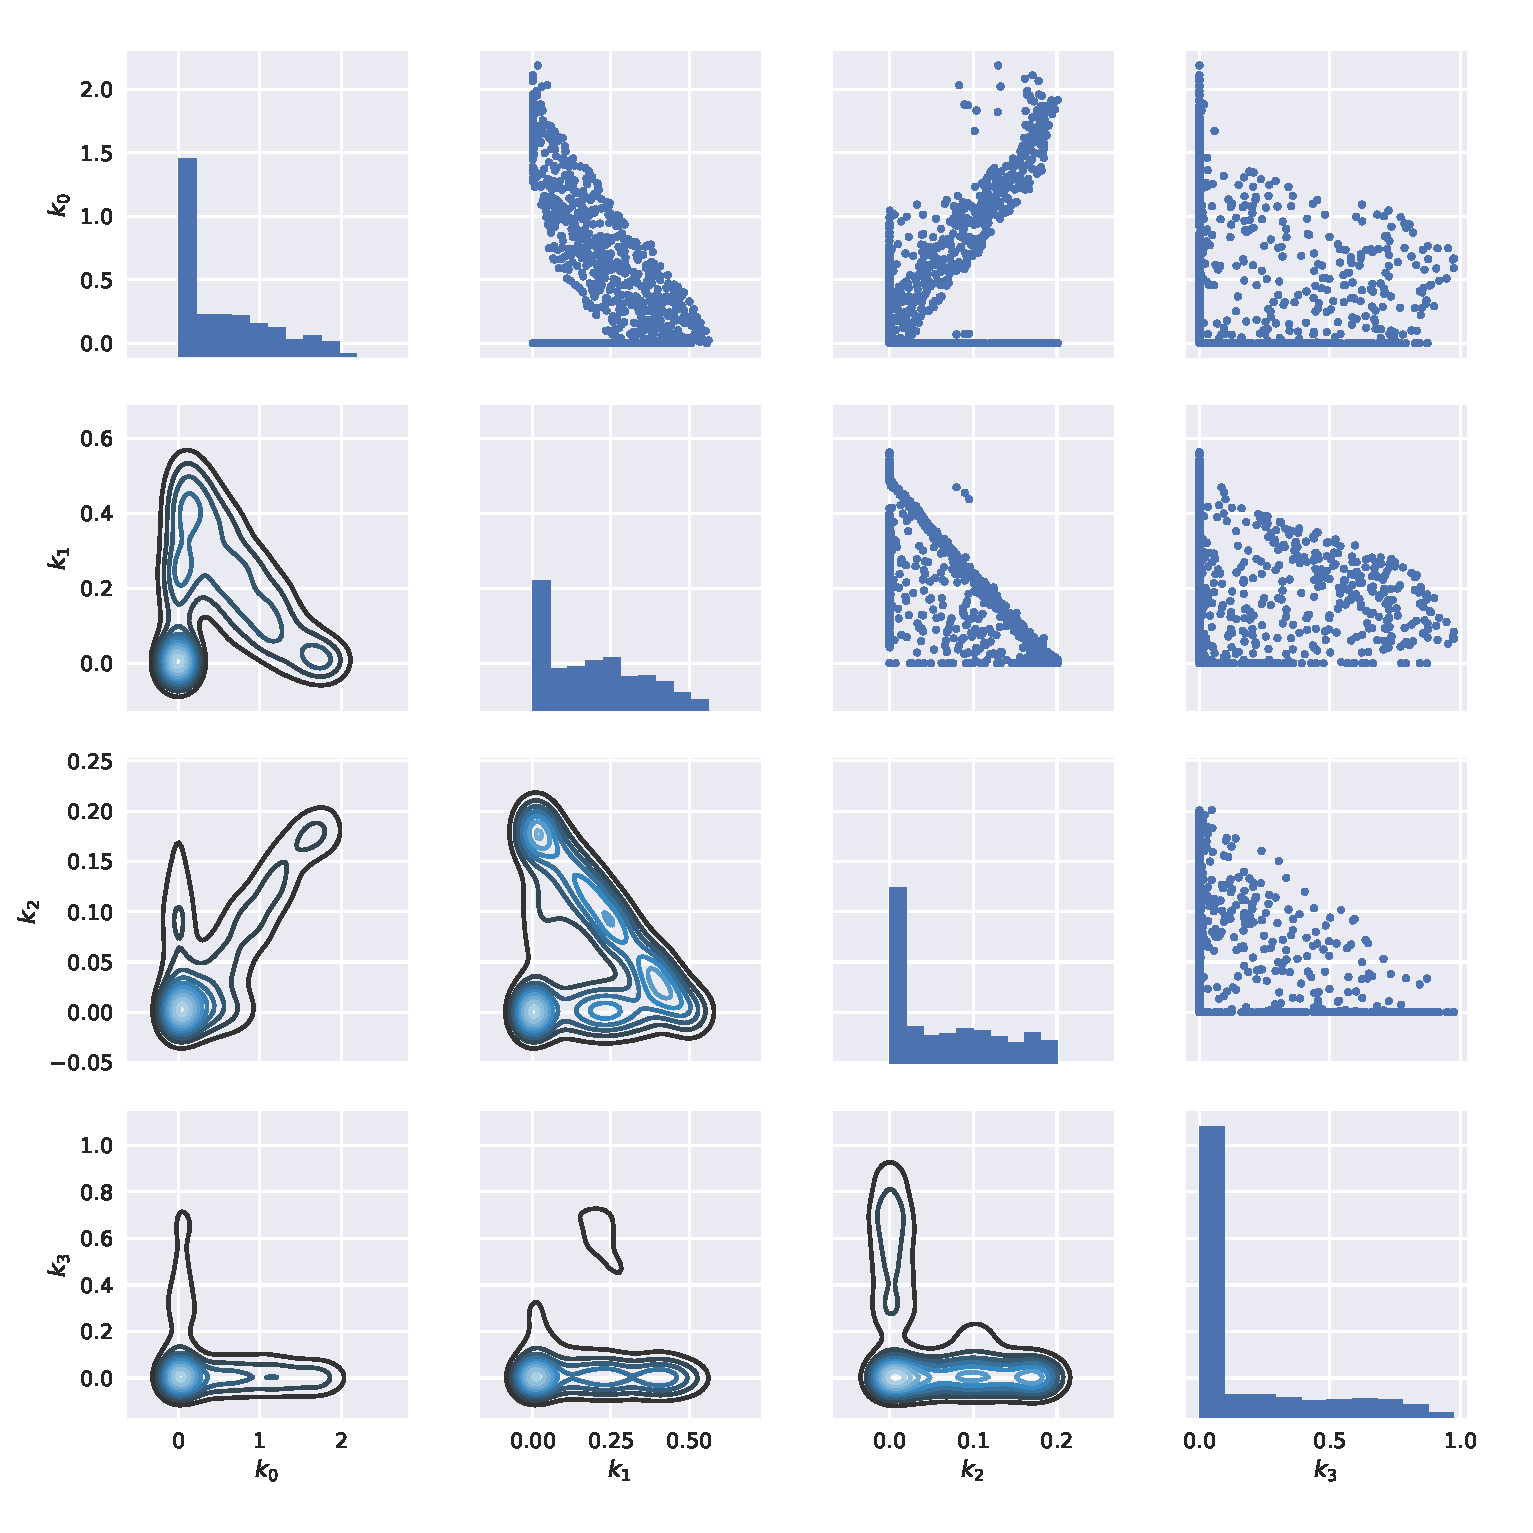
\includegraphics[width=0.8\linewidth]{pair_plot_4d_centered}
\end{figure}

% \begin{figure}[!h]
%   \centering
% 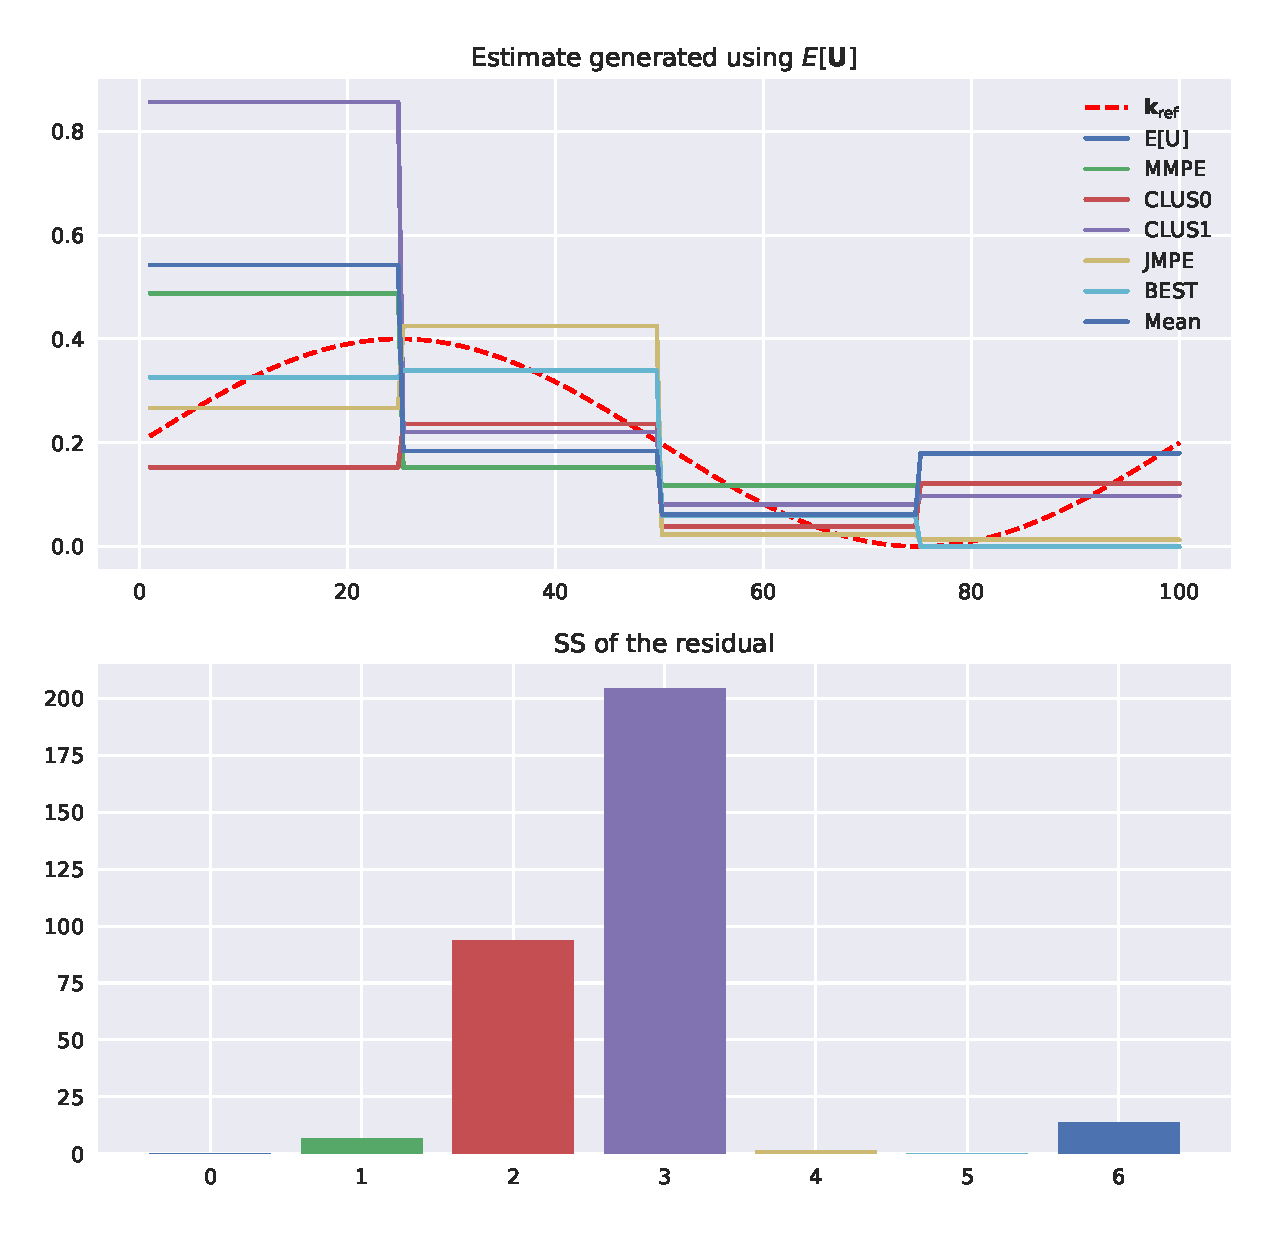
\includegraphics[width=0.85\linewidth]{estimate_centered}
% \end{figure}
\begin{figure}[!h]
  \centering
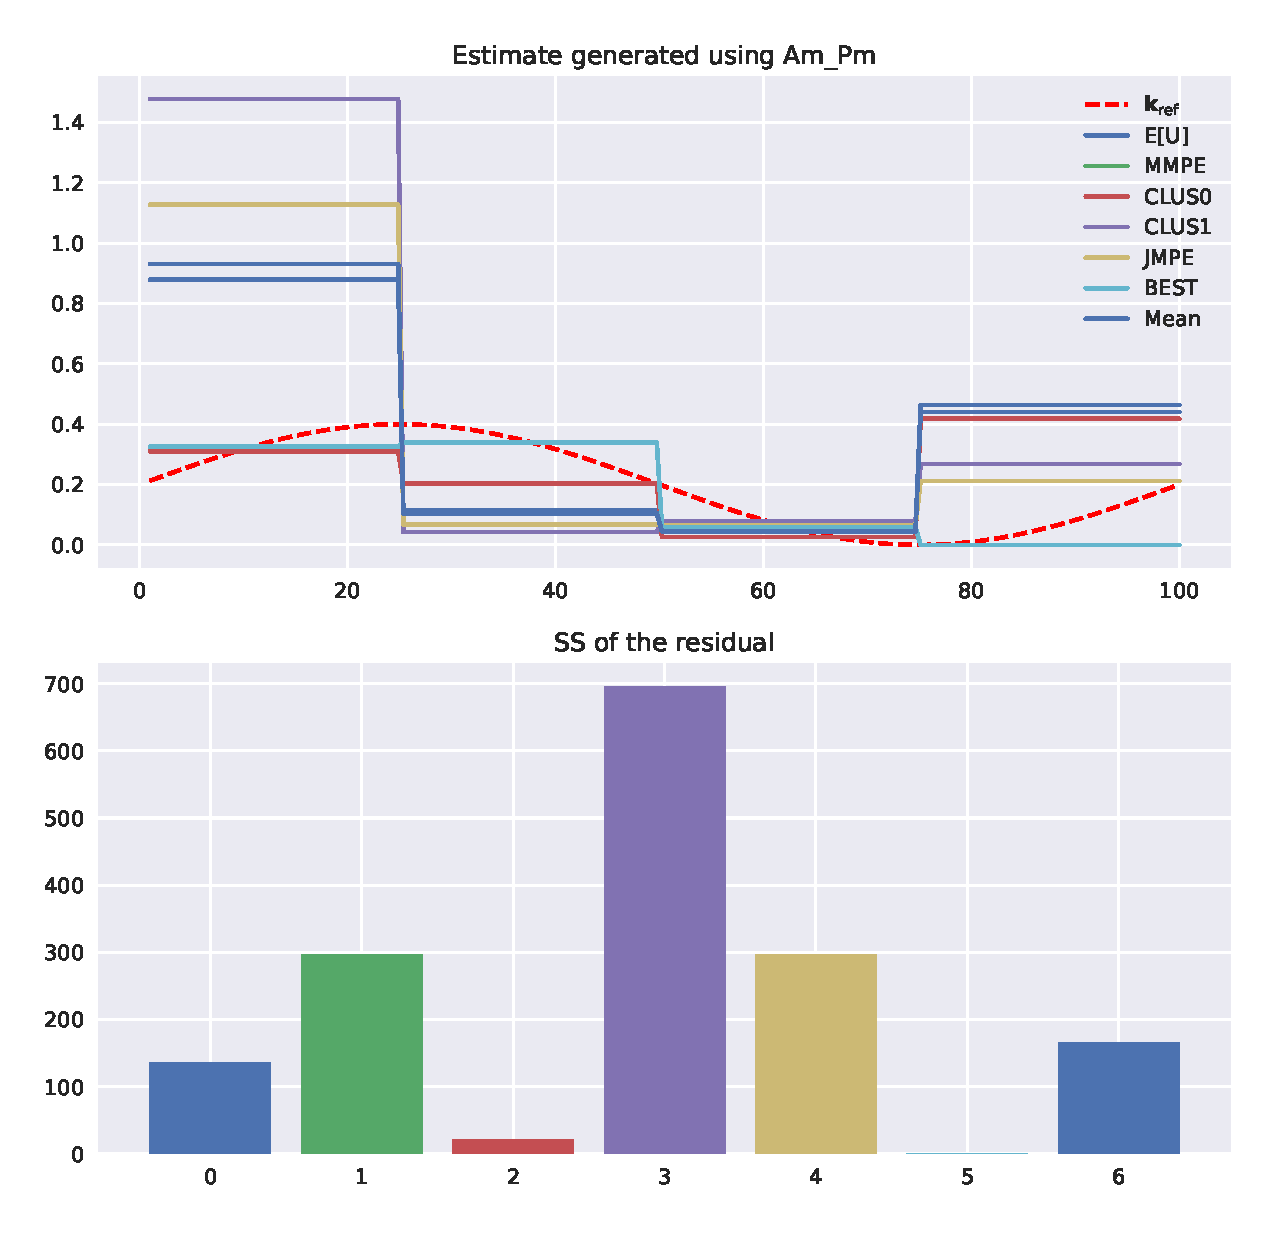
\includegraphics[width=0.85\linewidth]{estimate_Am_Pm}
\end{figure}

% \vspace{2ex}
% \begin{tabular}{l l l}
% \toprule
% \textbf{Treatments} & \textbf{Res. 1} & \textbf{Res. 2}\\
% \midrule
% Treatment 1 & 0.0003262 & 0.562 \\
% Treatment 2 & 0.0015681 & 0.910 \\
% Treatment 3 & 0.0009271 & 0.296 \\
% \bottomrule
% \end{tabular}
% \caption{Table caption}
% \end{table}

\end{block}


\begin{block}{Future Work/Perspectives}
  \begin{itemize}
  \item Use of \alert{Surrogate Models} ?
  \item \alert{Dimension reduction} of $\mathcal{K}$, $\mathcal{U}$
  \end{itemize}
\end{block}

%----------------------------------------------------------------------------------------
\begin{block}{References}
  {\scriptsize
  \bibliographystyle{unsrt} 
  \bibliography{../Documents/bibzotero}}
\end{block}


\end{column} % End of the second column

\begin{column}{\leftmar}
\end{column} % Empty spacer column

% \begin{column}{\onecolwid} % The third column

% %----------------------------------------------------------------------------------------
% %	CONCLUSION
% %----------------------------------------------------------------------------------------

% \begin{block}{Conclusion}

% Nunc tempus venenatis facilisis. \textbf{Curabitur suscipit} consequat eros non porttitor. Sed a massa dolor, id ornare enim. Fusce quis massa dictum tortor \textbf{tincidunt mattis}. Donec quam est, lobortis quis pretium at, laoreet scelerisque lacus. Nam quis odio enim, in molestie libero. Vivamus cursus mi at \textit{nulla elementum sollicitudin}.

% Nunc tempus venenatis facilisis. Curabitur suscipit consequat eros non porttitor. Sed a massa dolor, id ornare enim.

% \end{block}

% %----------------------------------------------------------------------------------------
% %	ADDITIONAL INFORMATION
% %----------------------------------------------------------------------------------------

% \begin{block}{Additional Information}

% Maecenas ultricies feugiat velit non mattis. Fusce tempus arcu id ligula varius dictum. 
% \begin{itemize}
% \item Curabitur pellentesque dignissim
% \item Eu facilisis est tempus quis
% \item Duis porta consequat lorem
% \end{itemize}

% Maecenas ultricies feugiat velit non mattis. Fusce tempus arcu id ligula varius dictum. 
% \begin{itemize}
% \item Curabitur pellentesque dignissim
% \item Eu facilisis est tempus quis
% \item Duis porta consequat lorem
% \end{itemize}

% \end{block}


% \end{column}

\end{columns}
\end{frame}
\end{document}
%%% Local Variables:
%%% mode: latex
%%% TeX-master: "<none>"
%%% End:
